\section*{Aufgabe 1}
\subsection*{Aufgabe 1a}
Für gleichverteilte Zahlen in einem Intervall $c$ bis $d$ ist die Wahrscheinlichkeit einen Wert $a$ zu ziehen genau so groß wie jeden beliebigen anderen Wert $b$. Dadurch ist die Wahrscheinlichkeit einen Wert zwischen $a$ und $b$ zu finden, gegeben durch:
\begin{align*}
  P(a \le x\le b) = \frac{b - a}{d - c}
\end{align*}
Wir haben nun ein Intervall von $c = 0$ bis $d = 1$ und einen Bereich zwischen $a = \frac{1}{3}$ und $b = \frac{1}{2}$ gegeben. Damit ist die Wahrscheinlichkeit eine Zahl aus diesem Bereich zu erhalten gleich:
\begin{align*}
  P\left(\frac{1}{3}\le x\le\frac{1}{2} \right) = \left(\frac{1}{2} - \frac{1}{3}\right) = \frac{1}{6}
\end{align*}

\subsection*{Aufgabe 1b}
Die Wahrscheinlichkeit einen exakten Wert aus einer gleichverteilten, kontinuierlichen Wahrscheinlichkeitsdichte zu ziehen geht gegen Null, weil es unendlich viele Werte in dem gegebenen Intervall gibt.

\subsection*{Aufgabe 1c}
Die kleinste positive Zahl, die sich mit 32 Bit (Single) darstellen lässt, kann über
\begin{align*}
  Z = \left(1.0 + \frac{M}{2^{23}}\right)\cdot 2^{E-127}
\end{align*}
bestimmt werden. Dafür muss $E = 0$ und $M = 1$ gewählt werden und es kommt $Z = 5.87747245476067 \cdot 10^{-39}$ raus. Diese Zahl entspricht auch der Wahrscheinlichkeit, dass der PC den exakten Wert $\frac{1}{2}$ findet.

\subsection*{Aufgabe 1d}
Die Wahrscheinlichkeit den exakten Wert von $\frac{2}{3}$ zu finden ist gleich null, weil $\frac{2}{3}$ unendlich viele Stellen hat. Allerdings wird $\frac{2}{3}$ im PC zu 0.6666666666666666 gerundet und dieser Wert kann mit der gleichen Wahrscheinlichkeit wie $\frac{1}{2}$ bestimmt werden.

\section*{Aufgabe 2}
\subsection*{Aufgabe 2b}
\begin{figure}
  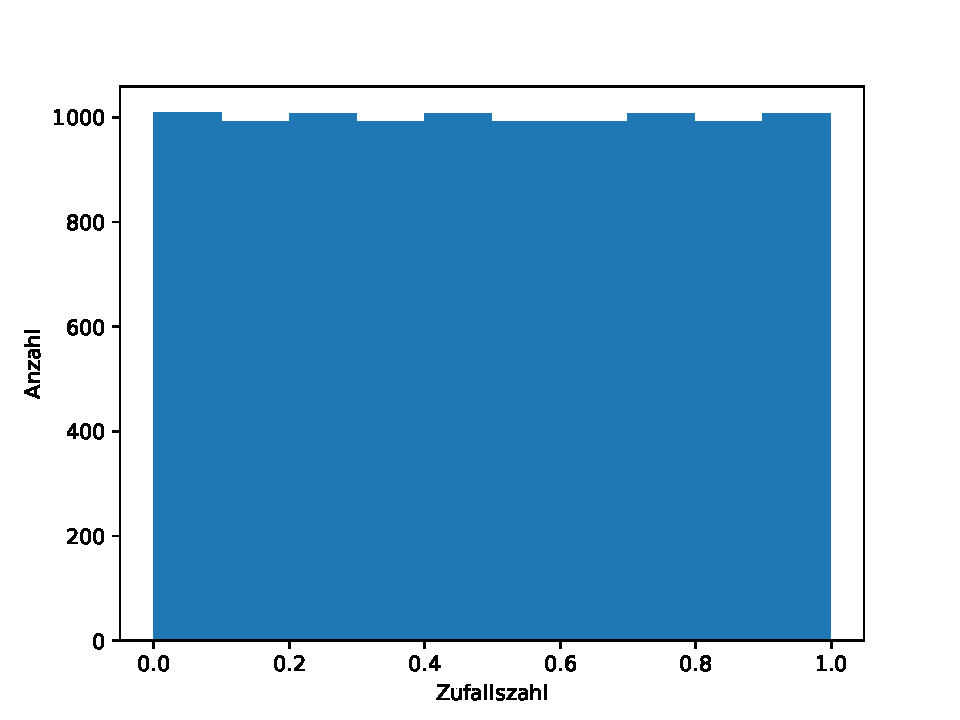
\includegraphics[height=10cm]{Python/Aufgabe2b.pdf}
  \caption{Histogramm von 10000 gleichverteilten Zahlen zwischen 0 und 1}
  \label{fig:2b}
\end{figure}
Der Zufallszahlengenerator hängt nicht bzw. nur vernachlässigbar vom Startwert ab.

\subsection*{Aufgabe 2c}
\begin{figure}
  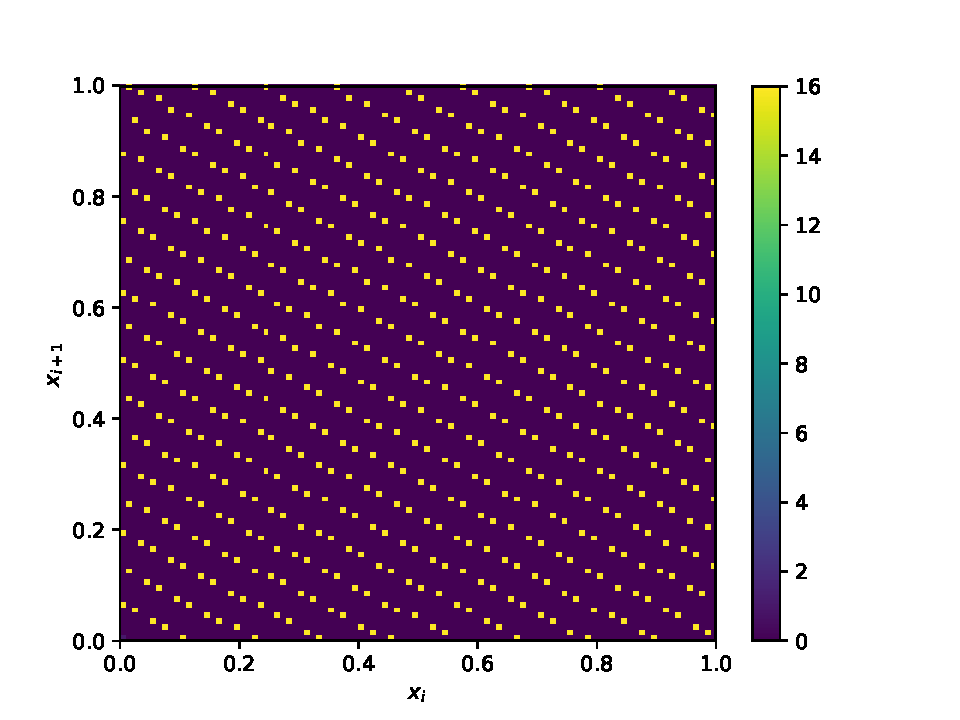
\includegraphics[height=10cm]{Python/Aufgabe2c1.pdf}
  \label{fig:2c1}
\end{figure}
\begin{figure}
  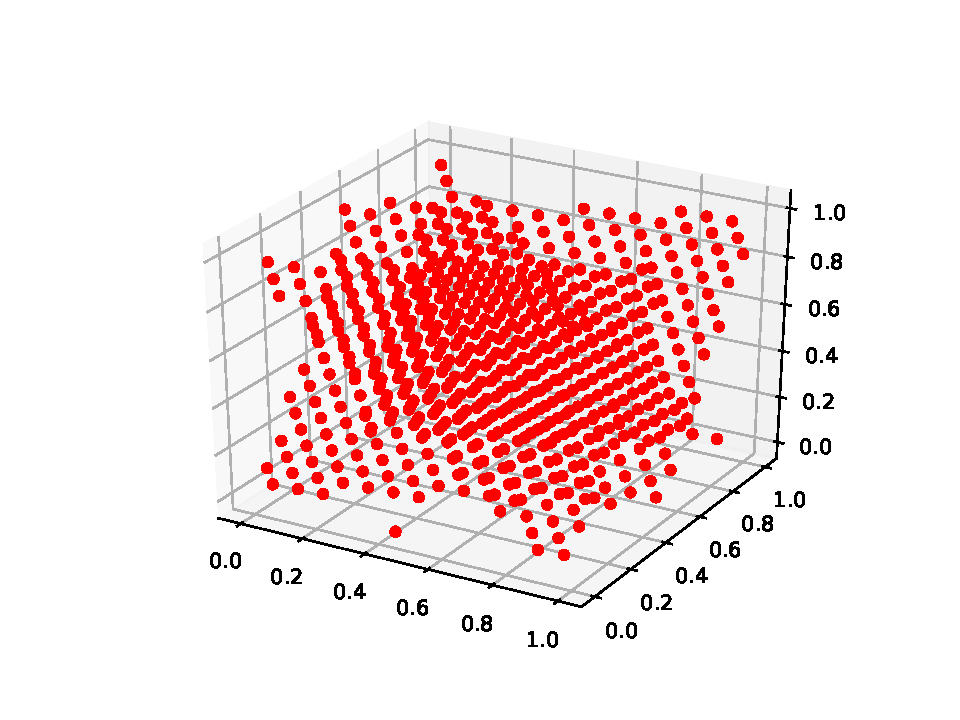
\includegraphics[height=10cm]{Python/Aufgabe2c2.pdf}
  \label{fig:2c2}
\end{figure}

Für einen guten Zufallsgenerator müssen im 2-dim Geraden und im 3-dim Ebenen mit gleicher Steigung und gleichem Abstand zueinander gegeben sein. \\
In Abbildung \ref{fig:2c1} sind deutlich Geraden mit gleichem Abstand und gleicher Steigung zu erkennen. \\ In Abbildung \ref{fig:2c2} kann man Ebenen erkennen, allerdings kann man nicht sagen ob diese parallel sind oder nicht. \\
Dennoch kann gesagt werden, dass es sich um einen guten Zufallsgenerator handelt.

\subsection*{Aufgabe 2d}
In der ROOT-Dokumentation zu TRandom.Rndm() steht, dass die Funktion ein Linear-kongruenter Zufallszahlengenerator ist, welcher gleichverteilte Zufallszahlen zwischen 0 und 1 ausgibt. Diese haben eine Periodizität von $2^{31}$. \\
Der von uns programmierte Zufallszahlengenerator gibt ebenfalls gleichverteilte Zufallszahlen aus, allerdings mit einer Periodizität von nur $625$.

\subsection*{Aufgabe 2e}
\begin{figure}[H]
  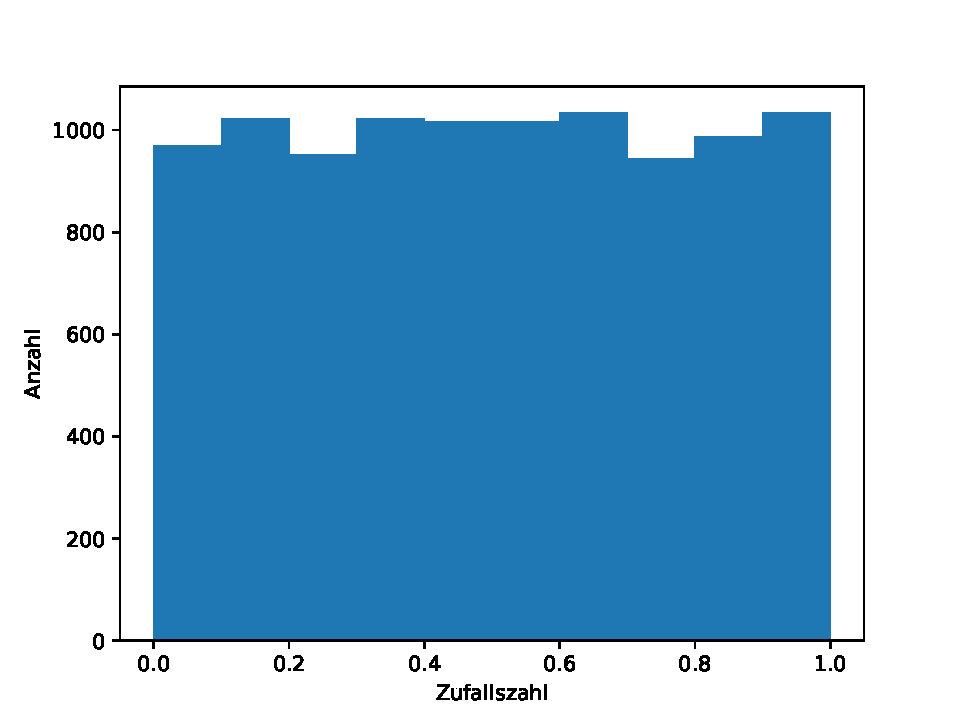
\includegraphics[height=11cm]{Python/Aufgabe2e1.pdf}
\end{figure}
\begin{figure}[H]
  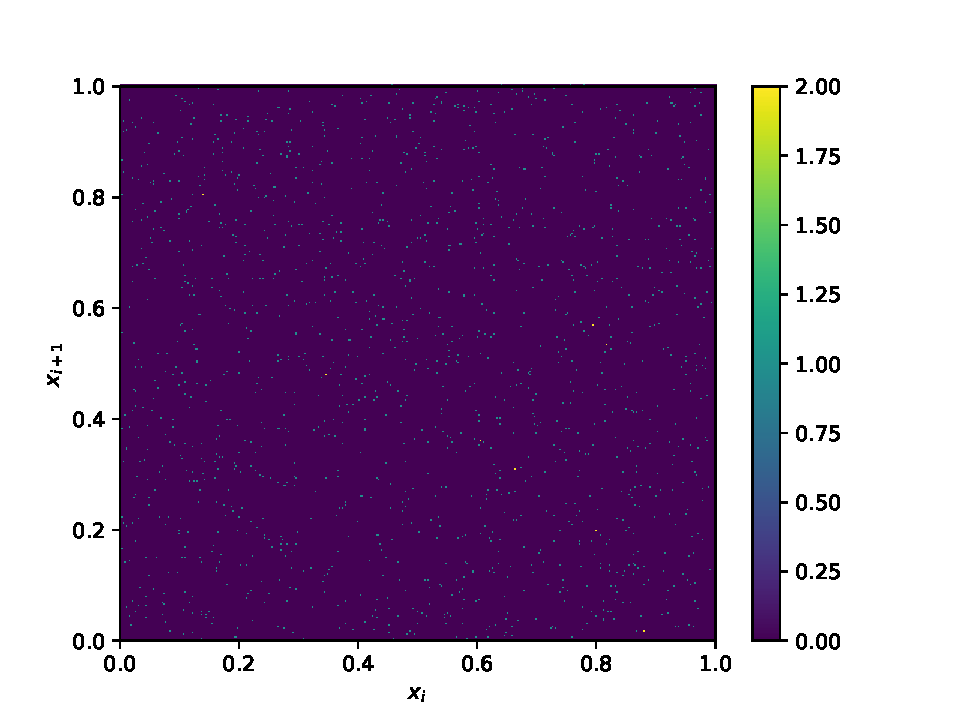
\includegraphics[height=10cm]{Python/Aufgabe2e2.pdf}
\end{figure}
\begin{figure}[H]
  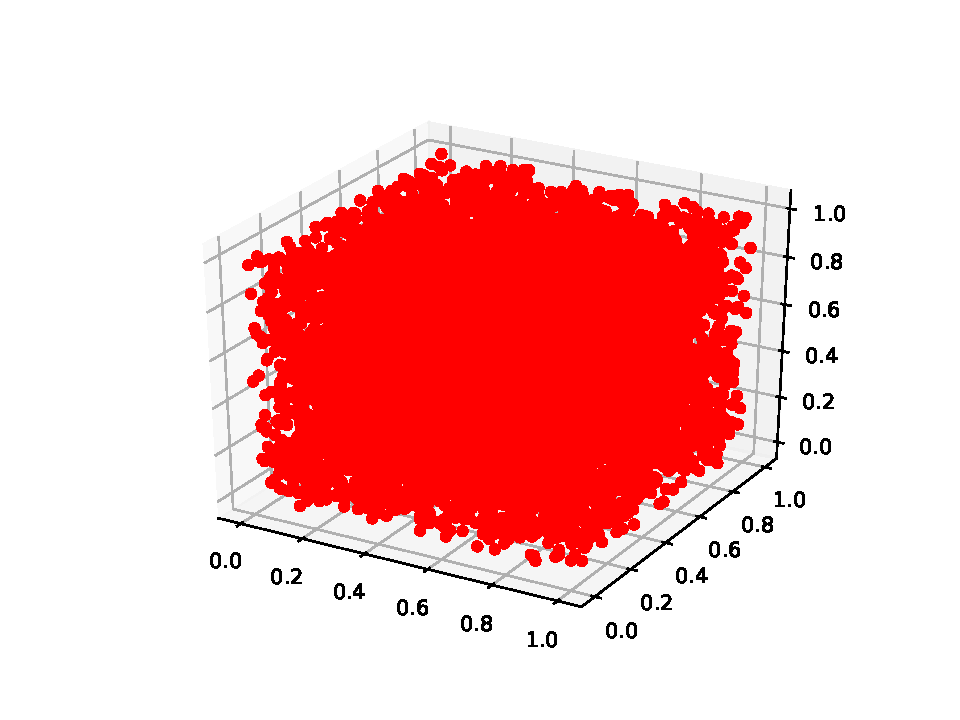
\includegraphics[height=10cm]{Python/Aufgabe2e3.pdf}
\end{figure}

\subsection*{Aufgabe 2f}
Die Funktion gibt bei einem Startwert von 5000 nach der Normierung 16-mal $\frac{1}{2}$ aus. Man kann mit jedem der 625 Werte die bei einem Startwert von 5000 auftauchen $\frac{1}{2}$ 16-mal erreichen. Daraus folgt, dass die Anzahl vom Startwert abhängt, denn wenn man keinen der 625 Werte nimmt, kann $\frac{1}{2}$ nicht erreicht werden.

\section*{Aufgabe 4}
\subsection*{Aufgabe 4a}
\begin{align*}
  f(x) = a_0 + a_1 \cdot x \\
  a_0 = \num{1.0 +- 0.2} \\
  a_1 = \num{1.0 +- 0.2} \\
  \rho = 0.8 \\
  \text{cov}(a_0, a_1) = \rho\,\sigma_{a_0}\,\sigma_{a_1} = 20
\end{align*}

unkorrelierte Fehlerfortpflanzung:
\begin{align*}
  \sigma_y &= \sqrt{\left(\frac{\partial f(x)}{\partial a_0}\ \sigma_{a_0} \right)^2 + \left(\frac{\partial f(x)}{\partial a_1}\ \sigma_{a_1} \right)^2} \\
  &= \sqrt{\sigma_{a_0}^2 + (x\,\sigma_{a_1})^2} = \sqrt{0.04\,x^2 + 0.04}
\end{align*}

korrelierte Fehlerfortpflanzung:
\begin{align*}
  \sigma_y &= \sqrt{\left(\frac{\partial f(x)}{\partial a_0} \sigma_{a_0} \right)^2 + \left(\frac{\partial f(x)}{\partial a_1} \sigma_{a_1} \right)^2 + 2\, \text{cov}(a_0, a_1) \left(\frac{\partial f(x)}{\partial a_0}\right) \left(\frac{\partial f(x)}{\partial a_1}\right)} \\
  &= \sqrt{\sigma_{a_1}^2\,x^2 + 1.6\,x + \sigma_{a_0}^2} = \sqrt{0.04\,x^2 + 40\,x + 0.04}
\end{align*}
